\subsection{Optimization of rates} % (fold)
\label{sub:optimization_of_rates}

    We solved optimization problems P1 and P2 for $\alpha \in \{0.01, 0.02, \ldots, 0.99\}$
    using $\mathbf{x^0} = [60~120~60~60~\mathbf{0}]^T$ and $\mathbf{x^d} =
    [0.5~2.5~1~1~0.5~1~1~1~57\alpha~57(1-\alpha)]^T$.  As Table I shows,
    the computed rates are constant for each $\alpha$ except for
    those corresponding to assembly and disassembly processes $4$ and $6$.
    This means that the system is flexible enough to yield any $\alpha$
    when only the rates of assembling and breaking apart the final
    assemblies are modified.  We also ran the Monte Carlo program
    for $\alpha=0.4$.  For the optimal set of rates, which were very similar to those for
    Problem P1, $t_{0.1} = 4.69$, as compared to $4.68$ for Problem P1 and $8.49$ for P2.  This
    provides evidence that Problem P1 is minimizing the system convergence time.



    \begin{table*}[t!]
        \begin{center}
        \caption{Values of optimized rates for varying $\alpha$. \textit{Continuous} rates
        evolve continuously with respect to $\alpha$.}
        \begin{tabular}{|c|c|c|c|c|c|c|}
            \hline
            \textbf{Reaction} $\mathbf{i}$ & \textbf{1} & \textbf{2} & \textbf{3} & \textbf{4} & \textbf{5} & \textbf{6} \\
            \hline
            \textbf{P1 Optimized} $\mathbf{p^+_i}$ & \multicolumn{6}{c|}{1.0} \\
            \hline
            \textbf{P1 Optimized} $\mathbf{p^-_i}$ & 0.01885 & 0.00754 & 0.00377 & \textit{continuous} & 0.00942 & \textit{continuous}\\
            \hline
            \textbf{P2 Optimized} $\mathbf{p^+_i}$ & 0.36 & 0.666 & 1.0 & \textit{continuous} & 0.4705 & \textit{continuous}\\
            \hline
            \textbf{P2 Optimized} $\mathbf{p^-_i}$ & 0.006855 & 0.005027 & 0.00377 & \textit{continuous} &  0.00443 & \textit{continuous} \\
            \hline
        \end{tabular}
        \end{center}
        \label{tab:optimized_rates}
    \end{table*}

     % ($k_4^-=0.0008269$, $k_6^-=0.0002205$)

%To verify the effect of the optimization on the system convergence,

We integrated the reduced macro-continuous model for $\alpha=0.4$
and $\alpha=0.8$ using the optimized rates from Problems P1 and P2
and a set of non-optimal rates that were chosen to satisfy
constraint \eqref{eq:equilConstr} and $\mathbf{0} \leq \mathbf{p}
\leq \mathbf{1}$ but were not optimized for some objective.  The
evolution of the model for each set of rates is shown in
Fig.~\ref{fig:ODEalpha_pt4}, with time in log-scale.  The optimized
systems first quickly converge to an ``intrinsic equilibrium" at $t
\approx 10^2$ that is independent of $\alpha$ and then redistribute
much more slowly to the target ratios, which are attained for all
set of rates.  For both $\alpha$, the optimized models converge
faster to equilibrium than the non-optimal model. For $\alpha=0.4$,
the non-optimal model displays a large over- and under-shooting of
the target ratios, whereas the optimized models converge quickly
with little or none of this effect.  Problem P2 produces a more
efficient system in this respect, although both optimized models
converge at comparable rates.

%Since the optimized models converge to the target ratio at
%comparable rates, \eqref{eq:obj1} and \eqref{eq:obj2} are both good
%objective functions

%Both objective functions used in Problems P1 and P2 seem good
%heuristics with respect to convergence time. Both have comparable
%performances, so we cannot decide between the two objectively.

%For $\alpha=0.4$, the non-optimal set of rates undergoes a flipping
%of ratios at $t=10^5$.


    \begin{figure}[!t]
        \centering
        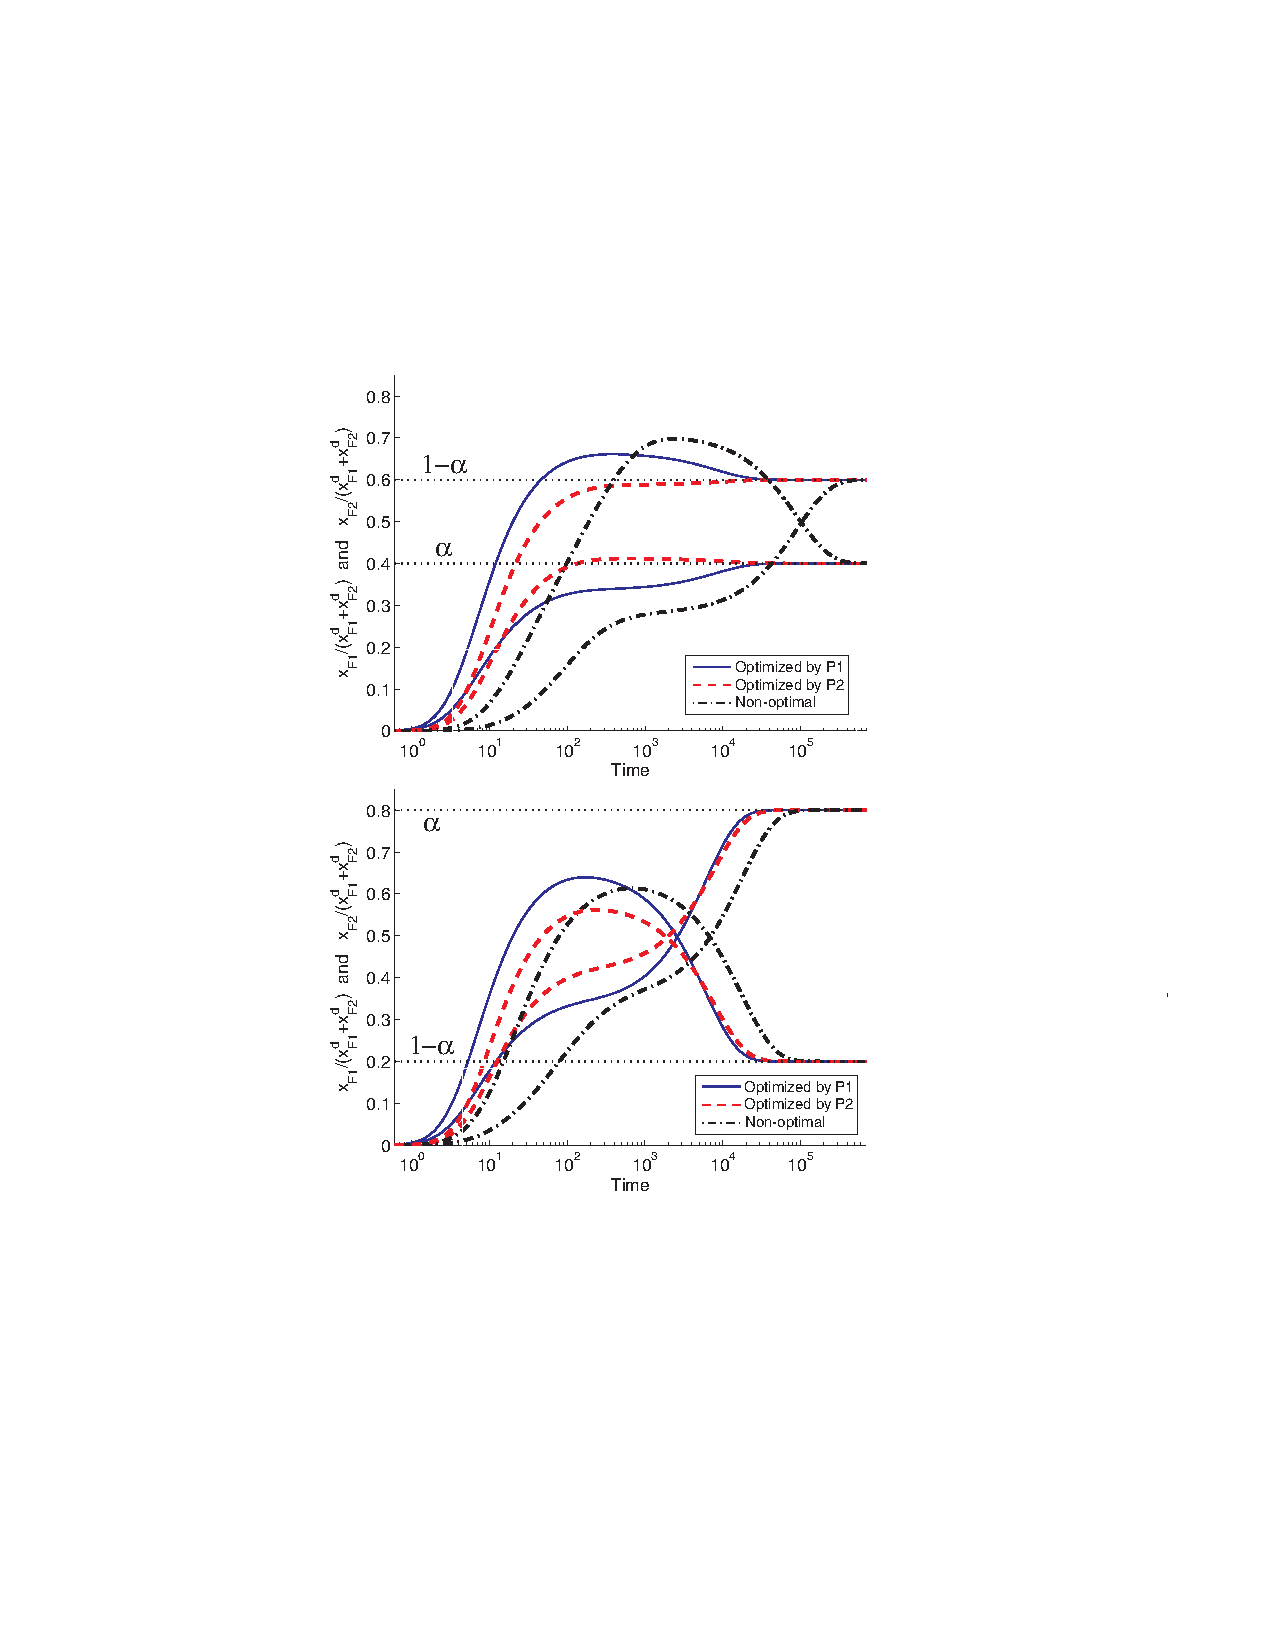
\includegraphics[trim= 40mm 75mm 10mm 60mm, clip,scale=0.65,angle=0]{img/ODE_alpha_comp2.pdf}
                %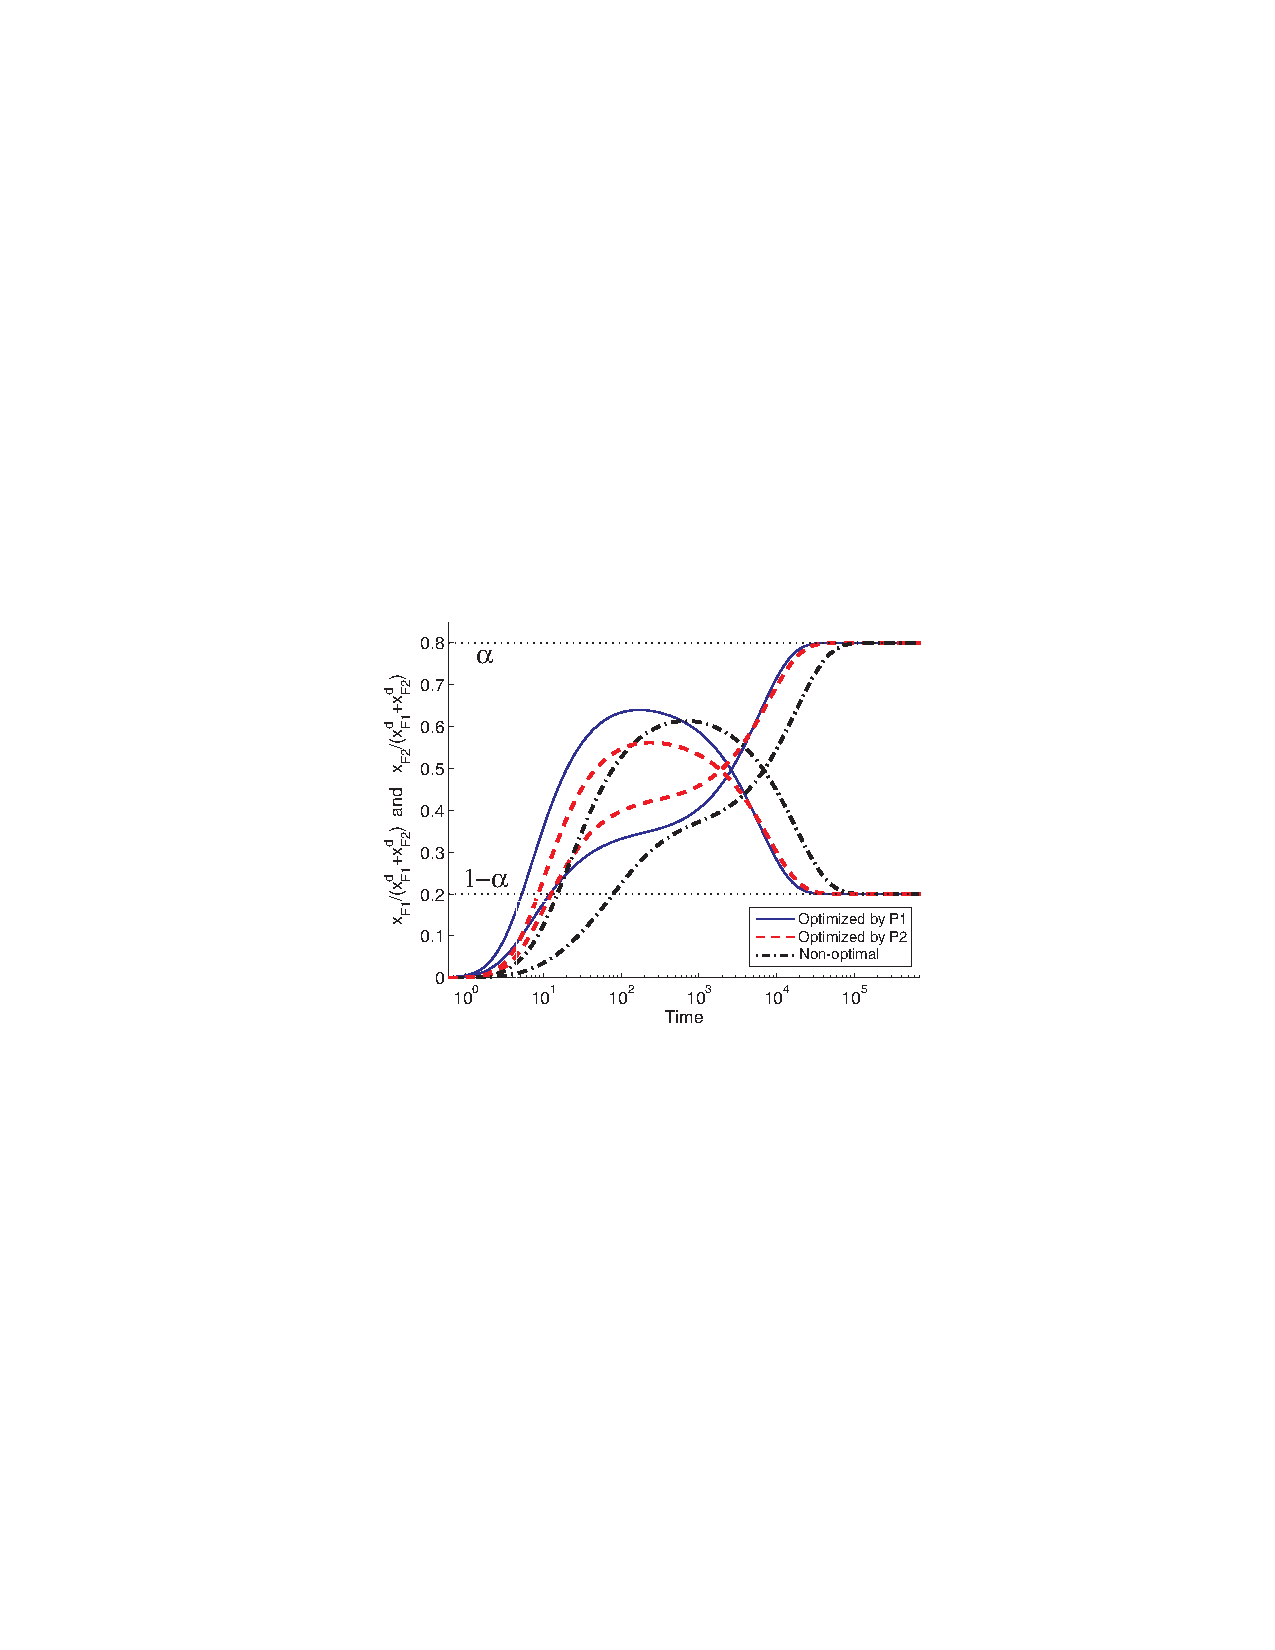
\includegraphics[trim= 70mm 85mm 70mm 85mm, clip,scale=0.7,angle=0]{img/ODE_alpha_comp_apt8.pdf}
        \caption{Evolution of final assembly ratios in the reduced macro-continuous model
         for $\alpha=0.4$ (top) and $\alpha = 0.8$ (bottom), using rates optimized by
         Problems P1 and P2 and non-optimal rates.}
        \label{fig:ODEalpha_pt4}
    \end{figure}


% subsection optimization_of_rates (end)

\subsection{Mapping rates onto the micro-continuous model} % (fold)
\label{sub:mapping_on_the_microscopic_model}

For $\alpha=0.4$, we mapped the rates optimized by Problem P1 and
the non-optimal rates onto the micro-continuous model to see whether
the physical system would behave similarly to the reduced continuous
model.  We did this in the following way.  Let $R$ be a uniformly
distributed random number between $0$ and $1$ and let $\Delta t$ be
the simulation timestep.  A robot carrying a part that can be
disassembled according to process $i$ computes $R$ at each timestep
and disassembles the part if $R < p_i^- \Delta t$. A robot about to
begin assembly process $i$ computes $R$ and executes the assembly if
$R < p_i^+ \Delta t$.  Fig.~\ref{fig:img_webots_results_alpha04}
shows the time evolution of the micro-continuous model averaged over
$30$ runs for both sets of rates, using $15$ robots and $15$ parts
($3$ final assemblies).  The non-optimal model converges to the
target ratios but initially over- and under-shoots $x_{F1}^d$ and
$x_{F2}^d$, respectively, as in Fig.~\ref{fig:ODEalpha_pt4}.  The
ratios in the optimized model rise quickly to the target ratios but
then deviate from them toward $0.5$.

%- I wanted to say that the convergence to the equilibrium is less
%stable. Actually the convergence is pretty bad if you look at it,
%but  I want to say that this is most likely because of variation
%around the  target ratios.

The discrepancy between the optimized model results and the target
ratios can be explained by inaccurate modeling of some low-level
effects.  In the micro-continuous model, when a robot disassembles a
part, a nearby robot is likely to pick up the fallen component and
quickly reassemble the original part with the other robot, which
generally hasn't traveled far.  This increases the rate of assembly
of the part and violates the well-mixed assumption.  In addition,
robots that pick up dropped parts spend a significant amount of time
carrying them before reassembly, a factor that was abstracted away
in the reduced model.  Adding more robots tends to alleviate this
effect.  Random failures at disassembly, incorrect internal state
definitions by the robots and parts, and collision errors by the
physics engine sometimes occur in the simulation but are not
modeled. Finally, the continuous abstraction may not accurately
capture the system behavior for such a low number of parts. However,
it becomes more computationally expensive to simulate the system as
the number of parts and robots increase.

%simulation speed decreases as the number of parts and robots
%increase.

%means that the number of final assemblies is small compared to the
%nonzero numbers of intermediate assemblies



    \begin{figure}[t]
        \centering
            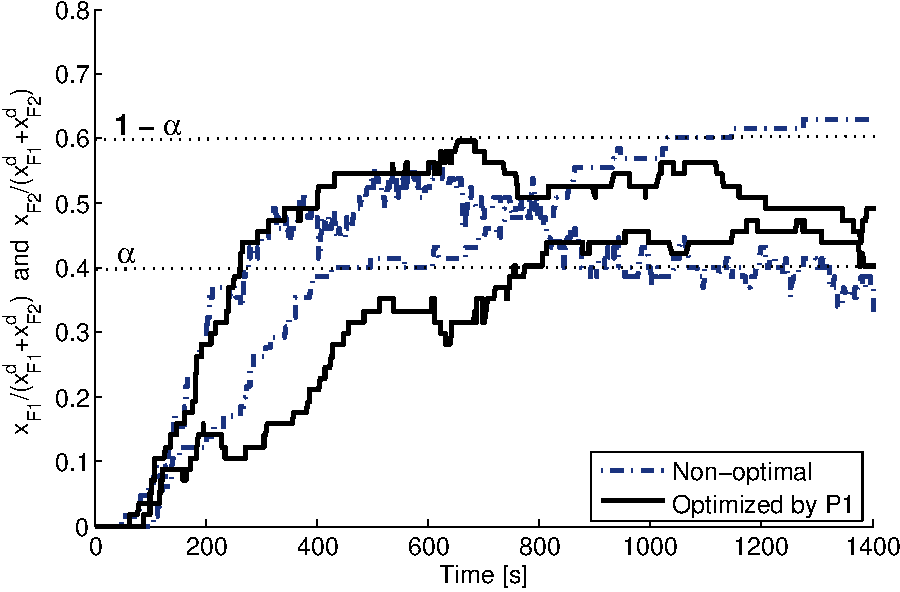
\includegraphics[width=8cm]{img/webots_results_alpha04.pdf}
        \caption{Evolution of final assembly ratios in the micro-continuous model
        for $\alpha=0.4$, using rates optimized by
         Problem P1 and non-optimal rates.}
        \label{fig:img_webots_results_alpha04}
    \end{figure}

% subsection mapping_on_the_microscopic_model (end)


\subsection{Reconfigurable manufacturing} % (fold)
\label{sub:green_manufacturing}

We apply our methodology to a ``green manufacturing" task, in which
finished products are recycled into new products in ratios that
depend on the current demand.  We perform a simulation of the
reduced macro-continuous model that corresponds to a situation in
which robots switch between sets of optimized rates at discrete
points in time to produce different target numbers of parts.  The
sequence of target $\alpha$ is $0.4, 0.99, 0.01$, and $0.5$, and
$\mathbf{x^0}$ is the same as in Section
\ref{sub:optimization_of_rates}.  The system evolution is shown in
Fig.~\ref{fig:img_optim_online_adaptation} using rates from Problem
P1.  The system quickly adapts to new target ratios, although some
take longer to attain than others (e.g. $\alpha=0.5$).  The results
demonstrate that high-level control of the system is possible in
real-time.

    %This high-order goal is directly realizable by changing abruptly the set of
    %reaction rates used by the robots.

    \begin{figure}[t]
        \centering
            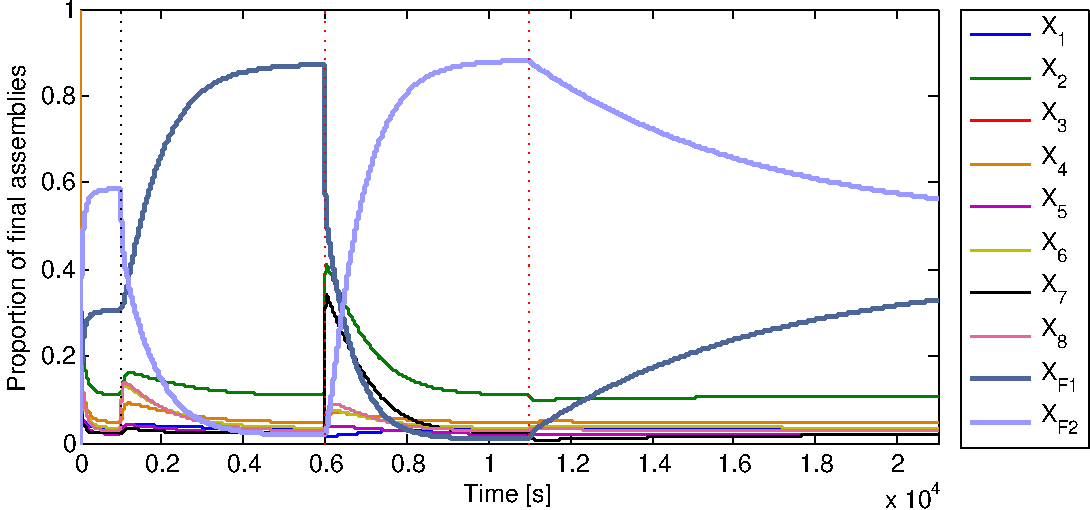
\includegraphics[width=8.5cm]{img/optim_online_adaptation.pdf}
        \caption{Online adaptation of the reduced macro-continuous model to changes in target equilibrium,
        which occur at the vertical dashed lines.}
        \label{fig:img_optim_online_adaptation}
    \end{figure}

% subsection green_manufacturing (end)
